\section{The Lorentz atom}
A Lorentz atom refers to the toy model of an atom where a single classical electron is harmonically bound to the nucleus, like a mass-spring.
\begin{figure}[htbp]
    \begin{subfigure}{.4\columnwidth}
        \centering
        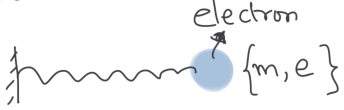
\includegraphics[width=\columnwidth]{PartOne/ChapterFour/figures/lorentzatom.png}
        \caption{Lorentz atom}
    \end{subfigure}
    \hfill
    \begin{subfigure}{.5\columnwidth}
        \centering
        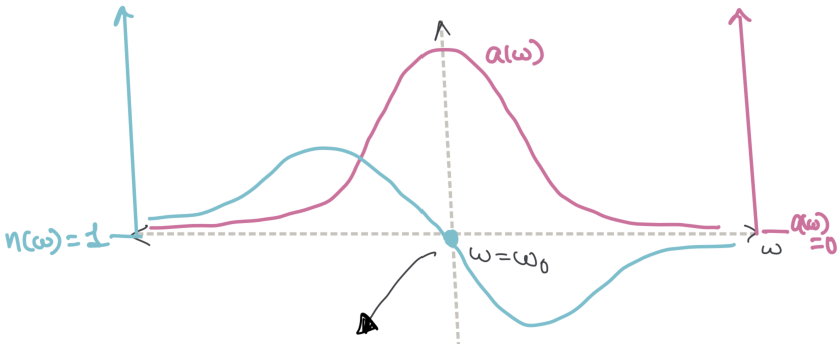
\includegraphics[width=\columnwidth]{PartOne/ChapterFour/figures/lorentzatom_refractiveindex.png}
        \caption{Refractive index behavior}
    \end{subfigure}
\end{figure}

Equation of motion for the electron is:
\begin{align}
    m\frac{d^2\br}{dt^2}+m\omega_0^2\br+2m\gamma\frac{d\br}{dt}=-e\bE(t),
\end{align}
where $\gamma$ is the frictional decay rate of oscilattory motion. The E-field and the induced position are:
\begin{align}
    \bE(t)=\sum_n\E_ne^{i\omega_nt}+\E^*_ne^{-i\omega_nt}\xrightarrow{\text{induced motion}}\br=\sum\left[\br_ne^{i\omega_nt}+\br_n^*e^{-i\omega_nt}\right].
\end{align}
By substituting both in the equation of motion and solving for $\br_n$ we find that:
\begin{align}
    \br_n=\left[-\frac{e}{m}\frac{1}{\omega_0^2-\omega_n^2+2i\gamma\omega_n}\right]\E_n.
\end{align}
The dipole moment of the atom induced by the E-field is:
\begin{align}
    \bd_n=-e\br_n=\alpha(\omega_n)\E_n=\frac{e^2}{m}\frac{1}{\omega_0^2-\omega_n^2+2i\gamma\omega_n}\E_n,\quad\alpha(\omega_n)=\text{polarizability of the atom}.
\end{align}
Therefore, the polarizability of the atom is:
\begin{align}
    \text{polarizability of the atom}\qquad\alpha(\omega_n)=\frac{e^2/m}{\omega_0^2-\omega_n^2+2i\gamma\omega_n}.
\end{align}
If the induced dipole moment for a single atom is $\bd$, for N atoms per uint volume we have:
\begin{align}
    \bP_n=N\bd_n=N\alpha(\omega_n)\E_n=\varepsilon_0\chi(\omega_n)\bE\longrightarrow\chi(\omega_n)=\frac{N\alpha(\omega_n)}{\varepsilon_0}.
\end{align}
Thus, the complex refractive index is:
\begin{align}
    \tilde{n}^2(\omega_n)=1+\chi(\omega_n)=1+\frac{N\alpha(\omega_n)}{\varepsilon_0}\longrightarrow\highlight{\tilde{n}(\omega_n)=\sqrt{1+\frac{N\alpha(\omega_n)}{\varepsilon_0}}}. 
\end{align}
As an EM-field passes through a medium it experiences:
\begin{itemize}[itemsep=0pt,topsep=0pt,parsep=0pt]
    \item Dispersion, defined by $\re{n(\omega)}$.\\
    \item Absorption, described by $\im{n(\omega)}$.
\end{itemize}
If $\chi(\omega_n)$ is small, we approximate above by the first-order of the square root:
\begin{align}
    \chi(\omega_n)\approx1+\frac{N\alpha(\omega_n)}{2\varepsilon_0}\Longrightarrow
    \begin{array}{l}
        \displaystyle n(\omega)=\re{\tilde{n}(\omega_n)}=
    1+\frac{Ne^2/m\varepsilon_0(\omega_0^2-\omega_n^2)}{2[(\omega_0^2-\omega_n^2)+4\omega_n^2\gamma^2]}\\
        \displaystyle a(\omega_n)=\im{\tilde{n}(\omega_n)}=\frac{-i\omega\gamma Ne^2/m\varepsilon_0}{[(\omega_0-\omega_n^2)^2+4\omega_n^2\gamma^2]}.
    \end{array}
\end{align} 
In the curve above both parts are plotted againd the frequency. At $\omega=\omega_0$ (resonance), the absorption is maximum whereas the dispersion is
minimum (vanishes).